\section{Clasificación de Eventos Físicos: \\ Eventos Task y Eventos Happening}
\label{sec:clasificacion_eventos_fisicos} 
Mediante un análisis de los eventos físicos de entrada y los eventos
físicos de salida se determinó su relación con la RdP. 

Se observa en la Figura~\ref{fig:actividades_evento_task} que una acción que
emite un evento físico de salida es desencadenada por decisiones tomadas
unilateralmente dentro del monitor de Petri.

La utilización de petición de ejecución como modo de sincronización (ver
sección~\ref{sec:sincronizacion_peticion_ejecucion}), posibilita realizar la
petición en cualquier momento, sin tener en cuenta el estado de la RdP. Por eso,
para todas aquellas acciones que emiten eventos físicos de salida, la petición
de ejecución se realiza tan pronto como sea posible al inicio de la ejecución del
programa. En consecuencia, en la Figura~\ref{fig:actividades_evento_task}, la
única condición para el inicio de ejecución es la decisión que se toma dentro
del monitor. Esto significa que la ejecución de dichas acciones depende
exclusivamente del estado actual de la red.

\begin{figure}[H]
	\centering
	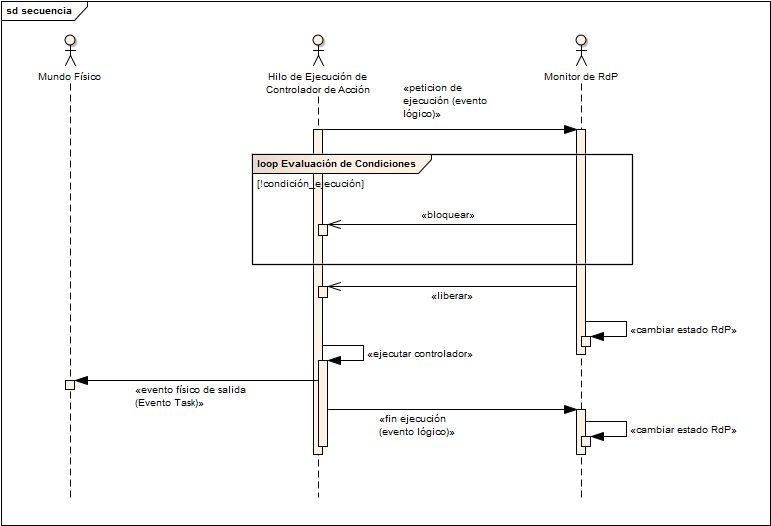
\includegraphics[width=120mm]{secuencia_evento_task}
	\caption{Diagrama de Secuencia de la Ejecución de una Acción que Emite un
	Evento Físico de Salida}
	\label{fig:actividades_evento_task}
\end{figure}

En cambio, en la Figura~\ref{fig:actividades_evento_happening} se observa que
una acción que se encarga de recibir y manejar un evento físico de entrada
depende en primera instancia de la ocurrencia de dicho evento. Luego, también es
sincronizada con la RdP mediante el uso del monitor. De este modo, las
acciones que reciben eventos físicos de entrada presentan una resticción extra
respecto a aquellas que emiten eventos físicos de salida.



\begin{figure}[H]
	\centering
	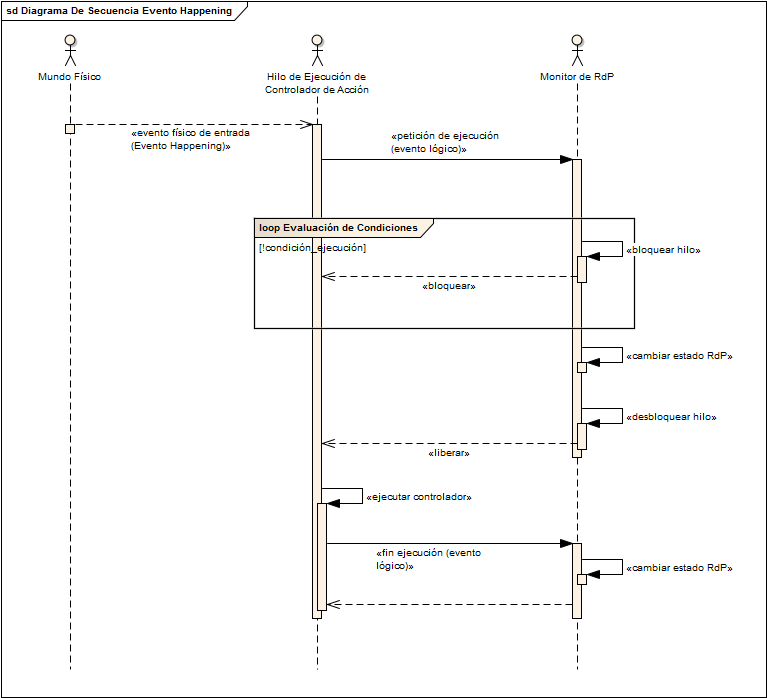
\includegraphics[width=120mm]{secuencia_evento_happening}
	\caption{Diagrama de Secuencia de la Ejecución de una Acción que Recibe un
	Evento Físico de Entrada}
	\label{fig:actividades_evento_happening}
\end{figure}

Desde este punto de vista, se decidió dar una clasificación más significativa a
los eventos físicos. Esta clasificación estará presente a lo largo de todo
el desarrollo del framework.
\begin{itemize}
  \item Eventos Task (Tarea): Eventos físicos de salida. Son
  desencadenados y sincronizados exclusivamente por eventos lógicos que dependen
  de condiciones ya presentes en el monitor de redes de petri al momento de su
  emisión. Si bien el monitor no produce directamente eventos físicos, puede
  advertirse que un evento task tiene una relación directa con determinados
  eventos lógicos. Dichos eventos lógicos se encuentran definidos en un tópico
  (evento de acción).
  \item Eventos Happening (Suceso): Eventos físicos de entrada. Son
  desencadenados por el mundo externo de manera totalmente asincrónica respecto
  al sistema. La ejecución de las acciones que reciben y manejan estos eventos
  es sincronizada por el monitor de redes de petri. De esta forma, el monitor
  conserva su responsabilidad frente al manejo del asincronismo del sistema.
  Los eventos lógicos requeridos para la sincronización se encuentran definidos
  en un tópico (evento de acción).
\end{itemize}

\section{Controladores de Acciones: \\ Task Controllers y Happening Controllers}
\label{sec:controladores_de_acciones}
Las acciones que debe realizar un sistema, junto con los mecanismos de
comunicación de los eventos físicos correspondientes, se encuentran embebidos
dentro de controladores de acción. Los mismos pueden observarse en la
Figura~\ref{fig:arquitectura_petri-manejador-acciones-mundo}. 
Luego de considerar lo expuesto en la
seccion~\ref{sec:clasificacion_eventos_fisicos}, surge la necesidad de
clasificar los controladores de acción respecto a su condición de receptores de
Eventos Happening, o de emisores de Eventos Task. Dicha clasificación
da origen a los controladores de tipo Happening Controller y Task
Controller respectivamente.

\subsection{Ejecución de un Task Controller}
\label{sec:ejecucion_task_controller}
De acuerdo a lo expuesto en la sección~\ref{sec:resumen_sincronizacion}, el 
modo de sincronización adoptado es el de petición de ejecución al monitor. 
De esta forma se admiten disparos asíncronos a transiciones realizados desde
diferentes hilos de ejecución, y el monitor se encarga de bloquear los hilos que
no pueden ejecutarse.
Otro concepto analizado en la seccion~\ref{sec:clasificacion_eventos_fisicos}
es que un Evento Task tiene una
relacion directa con determinados eventos lógicos. Además, un Evento Task es
desencadenado por condiciones que estan presentes en el monitor al momento de
la emisión de este evento. De esta forma, el comportamiento dinámico de los
Eventos Task será dirigido únicamente por la evolución de los estados de la red
de Petri.

Como corolario del analisis anterior se determina que la ejecución de un Task
Controller puede ser encapsulada en un hilo al momento de inicialización del programa.
El hilo se encarga de:
\begin{enumerate}
  \item Realizar las peticiones de los permisos de sincronización al
  monitor de forma directa, sin tener en cuenta el estado de la red.
  \item  Ejecutar el código correspondiente al Task Controller, una vez que el
  monitor otorga el permiso.
  \item  Realizar el aviso de finalización de ejecución al monitor de Petri.
  \item Repetir los pasos de ejecución de forma infinita, delegando en el
  monitor el control de la ejecución.
\end{enumerate}

La responsabilidad de la creación de los hilos para ejecutar los Task
Controllers pertenece al framework. En consecuencia, la ejecución de las
acciones encapsuladas en un Task Controller es transparente al usuario
desarrollador.

\begin{figure}[H]
	\centering
	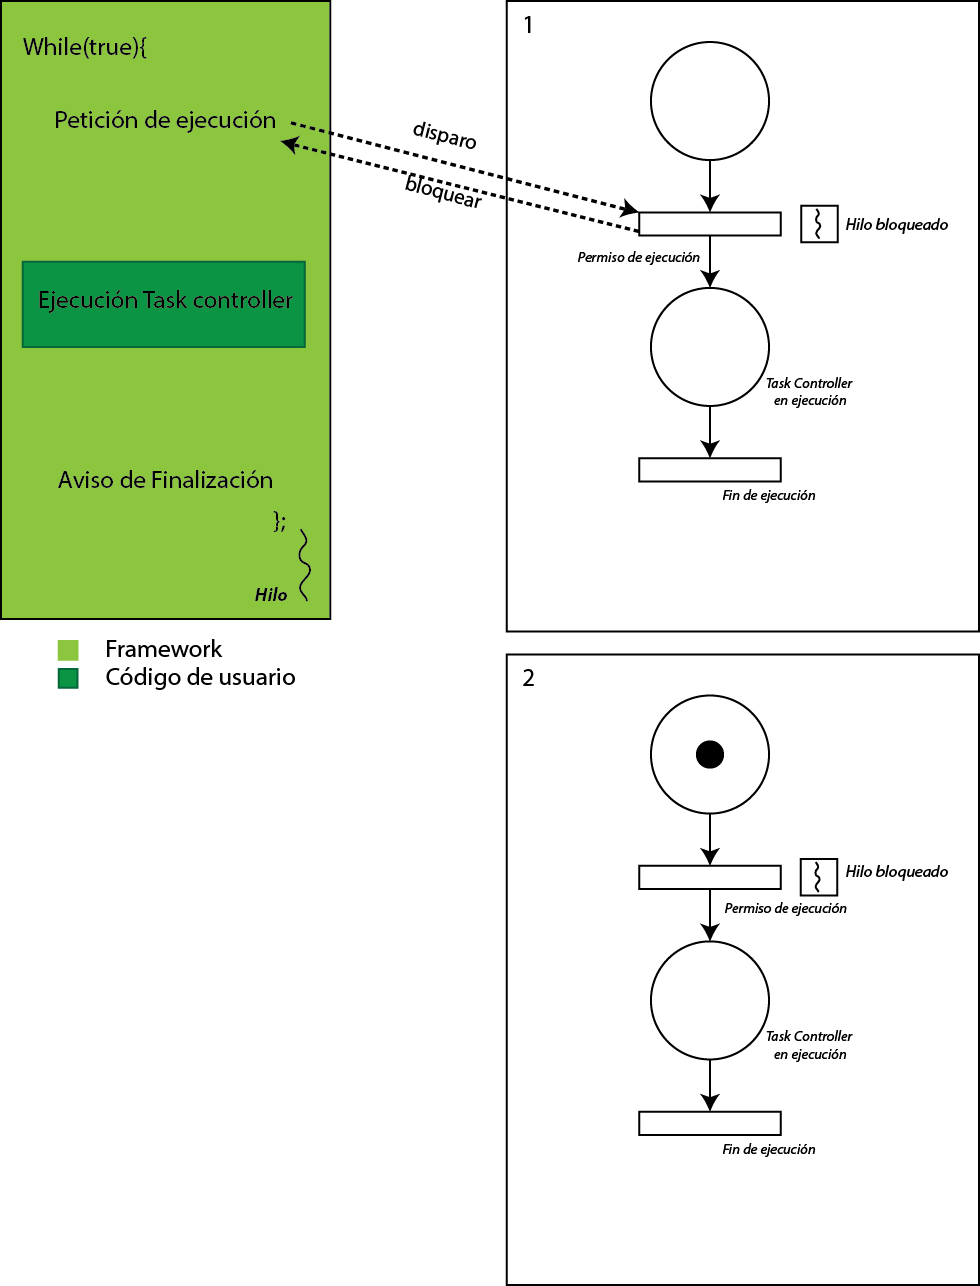
\includegraphics[width=120mm]{ejecucion_task_controller_pt1}
\end{figure}
\begin{figure}[H]
	\centering
	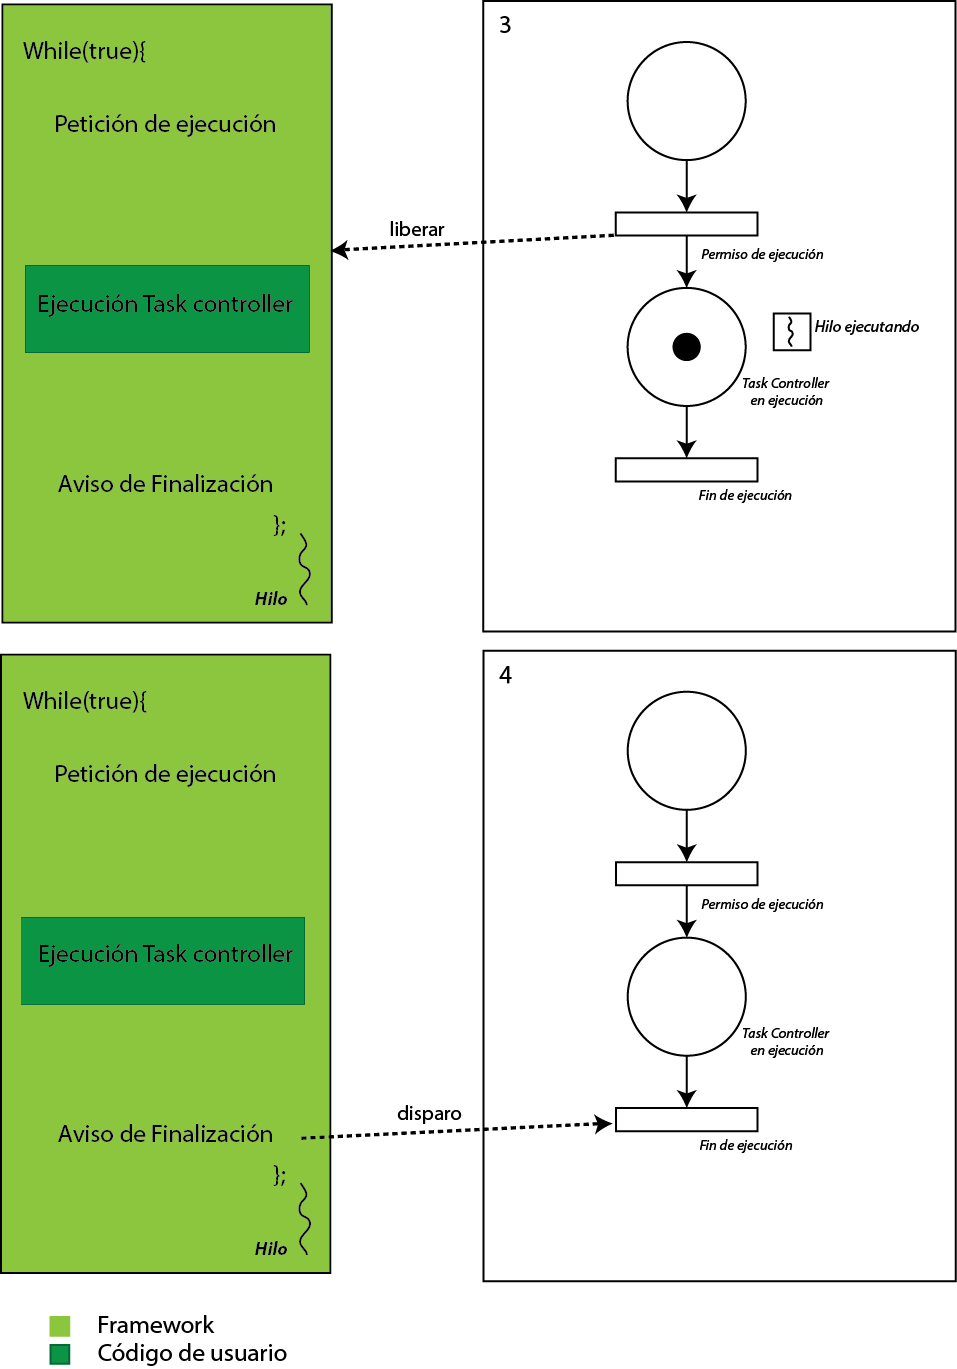
\includegraphics[width=120mm]{ejecucion_task_controller_pt2}
	\caption{Pasos de la Ejecución de un Task Controller}
	\label{fig:ejecucion_task_controller}
\end{figure}

\newpage

\subsection{Ejecución de un Happening Controller}
\label{sec:ejecucion_happening_controller}
En la seccion~\ref{sec:clasificacion_eventos_fisicos} se explica que un Evento
Happening se desencadena en el mundo externo y de forma asíncrona al sistema. 
En consecuencia, el código de usuario es quien realiza la llamada a ejecución
de un Happening Controller encargado de manejar dicho evento.

En principio, realizar una llamada desde el código de usuario podría generar un
grave problema en cuanto a las responsabilidades de sincronización. Las
acciones del Happening Controller quedarían fuera del mecanismo de
sincronización del monitor de Petri, atentando contra el objetivo de delegar
el asincronismo del sistema en la RdP.
Este problema es resuelto mediante la utilización de herramientas de la
programacón orientada a aspectos (ver sección~\ref{sec:aop}). Se optó por
encapsular las instrucciones de sincronización necesarias dentro de advices que
responden a joinpoints definidos por la ejecución de Happening Controllers.

\begin{framed}
\textbf{Nota:}
	Un controlador de acción que reacciona ante
	eventos Happening (Happening Controller) debe ser ejecutado dentro del
	contexto de un Listener u Observer del evento deseado.
	Para maximizar las libertades de elección del desarrollador en la recepción de
	eventos externos, la responsabilidad de crear estos Listeners se delega en el
	usuario.
\end{framed}


El flujo de ejecución de un Happening Controller es el siguiente:
\begin{enumerate}
  \item Cuando el código de usuario hace un llamado a la ejecución del Happening
  Controller, la aplicación alcanza un joinpoint.
  \item En el momento en que se alcanza el joinpoint se aplica un advice que
  realiza los pedidos de permiso de sincronización al monitor. Dicho advice es
  aplicado automáticamente en tiempo de compilación, por lo tanto el usuario no
  tiene la responsabilidad de realizar la sincronización manualmente. De esta
  manera se logra conservar la inversión de control.
  \item Una vez que el monitor libera el hilo, indicando que la ejecución es
  posible, se procede a ejecutar el código del controller.
  \item Al finalizar la ejecución del Happening Controller, se alcanza un nuevo
  joinpoint.
  \item En el momento en que se alcanza el joinpoint descripto en el punto
  anterior se aplica un advice que realiza el aviso de finalización de
  ejecución al monitor. Este advice se aplica de manera análoga a la descripta
  en el punto 2.
\end{enumerate}

\begin{framed}
\textbf{Nota:} Los advices descriptos en esta sección son ejecutados por el
mismo hilo que ejecuta el código del Happening Controller. Dado que la llamada
al código del Happening Controller es responsabilidad del usuario, es él quien
debe generar el hilo encargado de ejecutar el código. Se recomienda no utilizar
el hilo principal del programa para ejecutar Happening Controllers ya que puede
llevar al bloqueo del sistema.
\end{framed}

En conclusión, la sincronización de la ejecución de los Happening Controllers
sigue siendo una responsabilidad del monitor y es realizada de forma
transparente al usuario. Además, el usuario tiene total libertad para que el
Happening Controller reaccione ante un evento físico de entrada, permitiendo
que la llamada se realice en cualquier punto de la aplicación. Se debe destacar
que si bien el usuario tiene la libertad de llamar al código del Happening
Controller en cualquier momento, es el monitor quién determina si la
ejecución será en el momento de la llamada o si el hilo debe ser
bloqueado por no cumplirse las condiciones para su ejecución.

\begin{figure}[H]
	\centering
	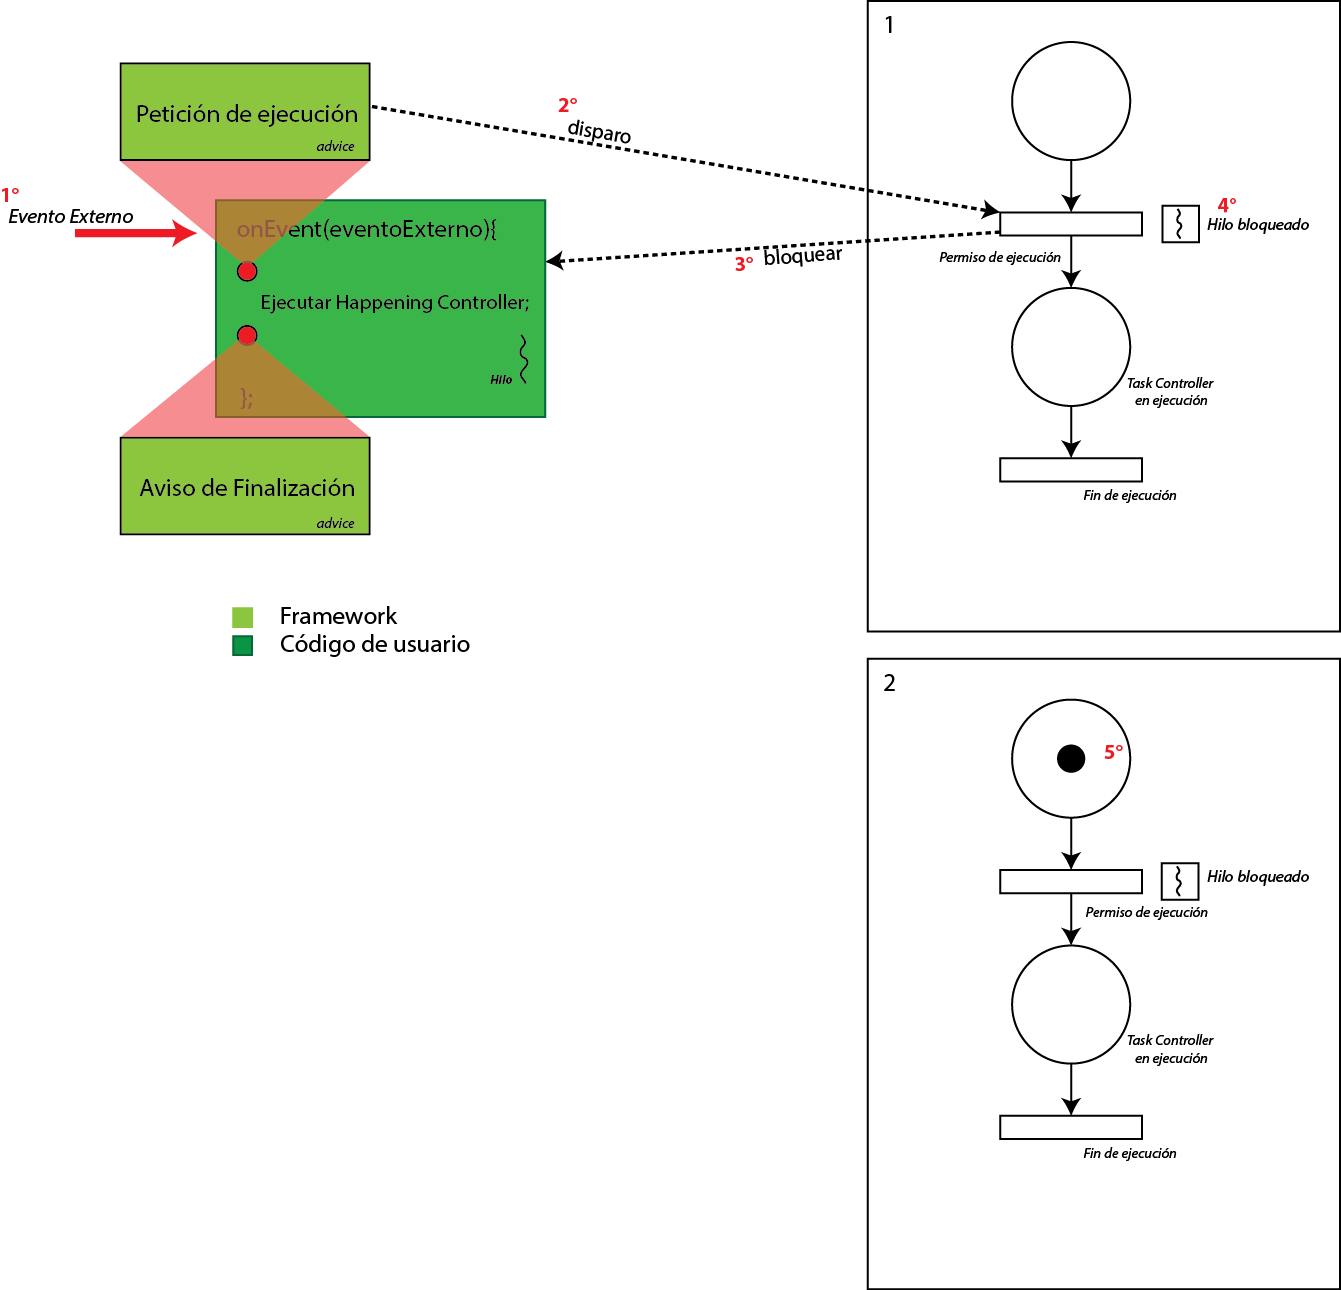
\includegraphics[width=120mm]{ejecucion_happening_controller_pt1}
\end{figure}
\begin{figure}[H]
	\centering
	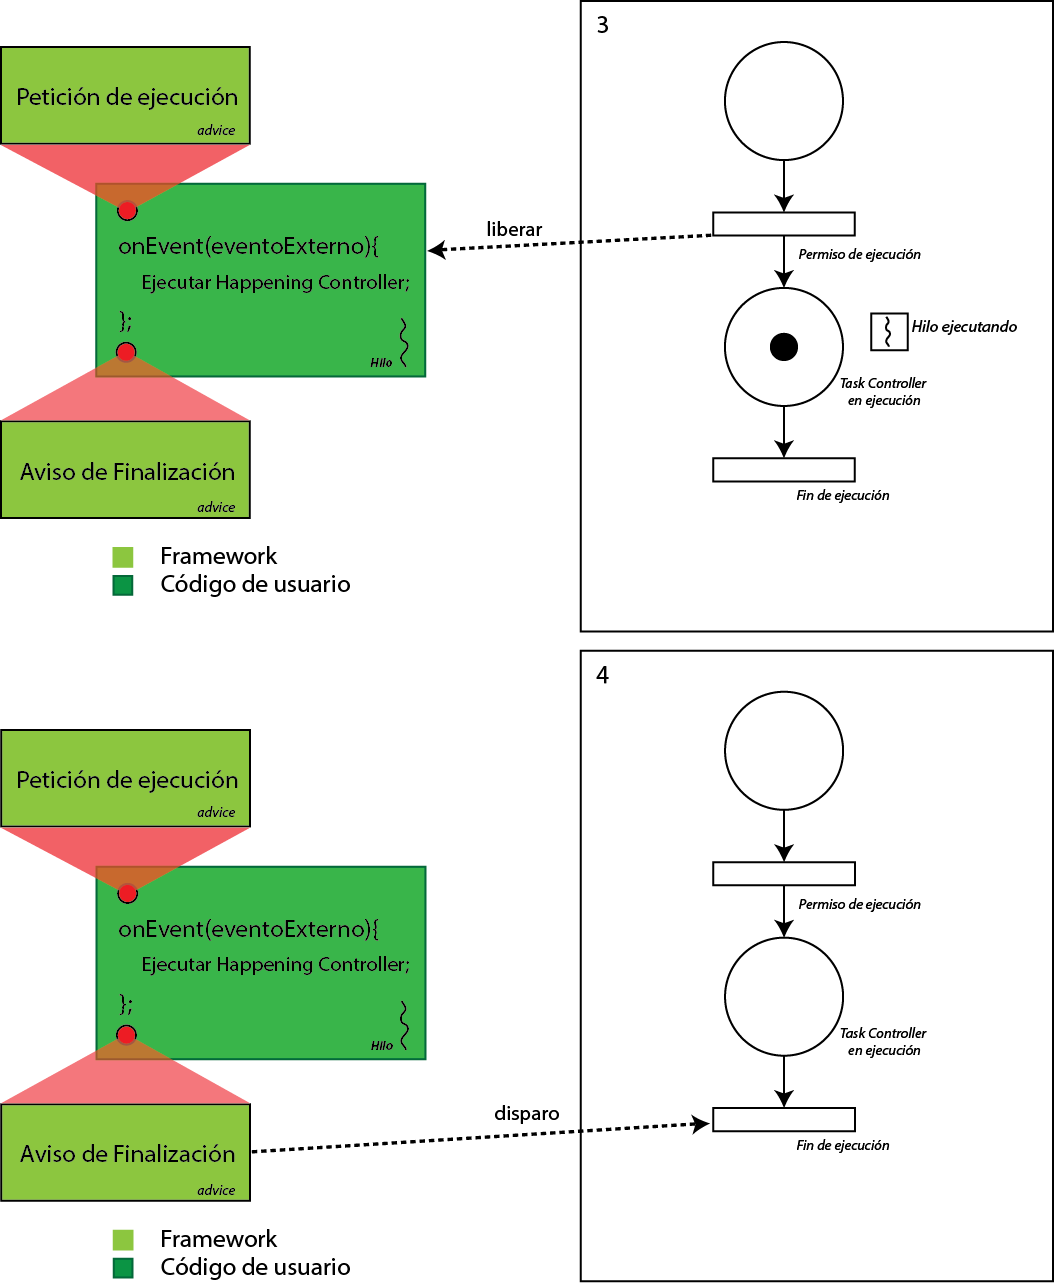
\includegraphics[width=120mm]{ejecucion_happening_controller_pt2}
	\caption{Pasos de la Ejecución de un Happening Controller}
	\label{fig:ejecucion_happening_controller}
\end{figure}

\section{ComplexSecuentialTaskController}
\label{sec:complex_secuential_task_controller}
La ejecución de un Task Controller, definida en la
sección~\ref{sec:ejecucion_task_controller}, puede optimizarse para sistemas (o
partes de sistemas) de caracter secuencial, como el que se estudia en la
sección~\ref{sec:sincronizacion_cinta_transportadora}.
Esto se debe a que no existe un paralelismo aprovechable en una secuencia de
tareas dependientes, por lo que resulta innecesario utilizar un hilo
por cada Task Controller correspondiente a cada tarea secuencial.

Se propone que aquellos Task Controllers de acciones
correspondientes a un proceso secuencial sean ejecutados por un mismo hilo .
Dicha agrupación es denominada Complex Secuential Task Controller. De esta
manera, se reduce una gran parte de los hilos necesarios para ejecutar un
sistema con tareas secuenciales.
Para lograrlo, se incorpora una etapa de petición de permisos y una etapa de
ejecución de controlador por cada Task Controller que forma parte del
ComplexSecuentialTaskController. Cada una de estas etapas debe seguir el orden
preestablecido por la secuencia de acciones que conforman el proceso secuencial.
Dicho orden se establece en el tópico, al definir el evento de acción para la
sincronización de la tarea compleja.

Una gran ventaja de agrupar tareas
secuenciales en un mismo hilo es que permite eliminar la plaza-transición incorporada por el Modo de
Sincronización de petición de de ejecución (ver
sección~\ref{sec:sincronizacion_peticion_ejecucion_transicion_plaza}).

\begin{figure}[H]
	\centering
	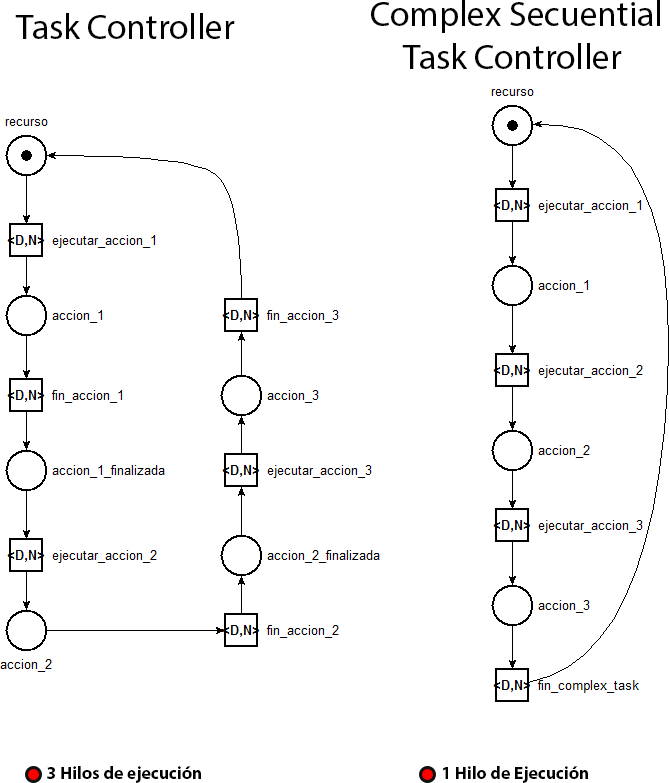
\includegraphics[width=120mm]{simple_vs_complex_task_petri_net}
	\caption{Comparación del modelo en RdP de un sistema con tres
	acciones secuenciales para Task Controllers simples y para Complex Secuential
	Task Controller.}
	\label{fig:simple_task_vs_complex_task_petri_net}
\end{figure}

\begin{figure}[H]
	\centering
	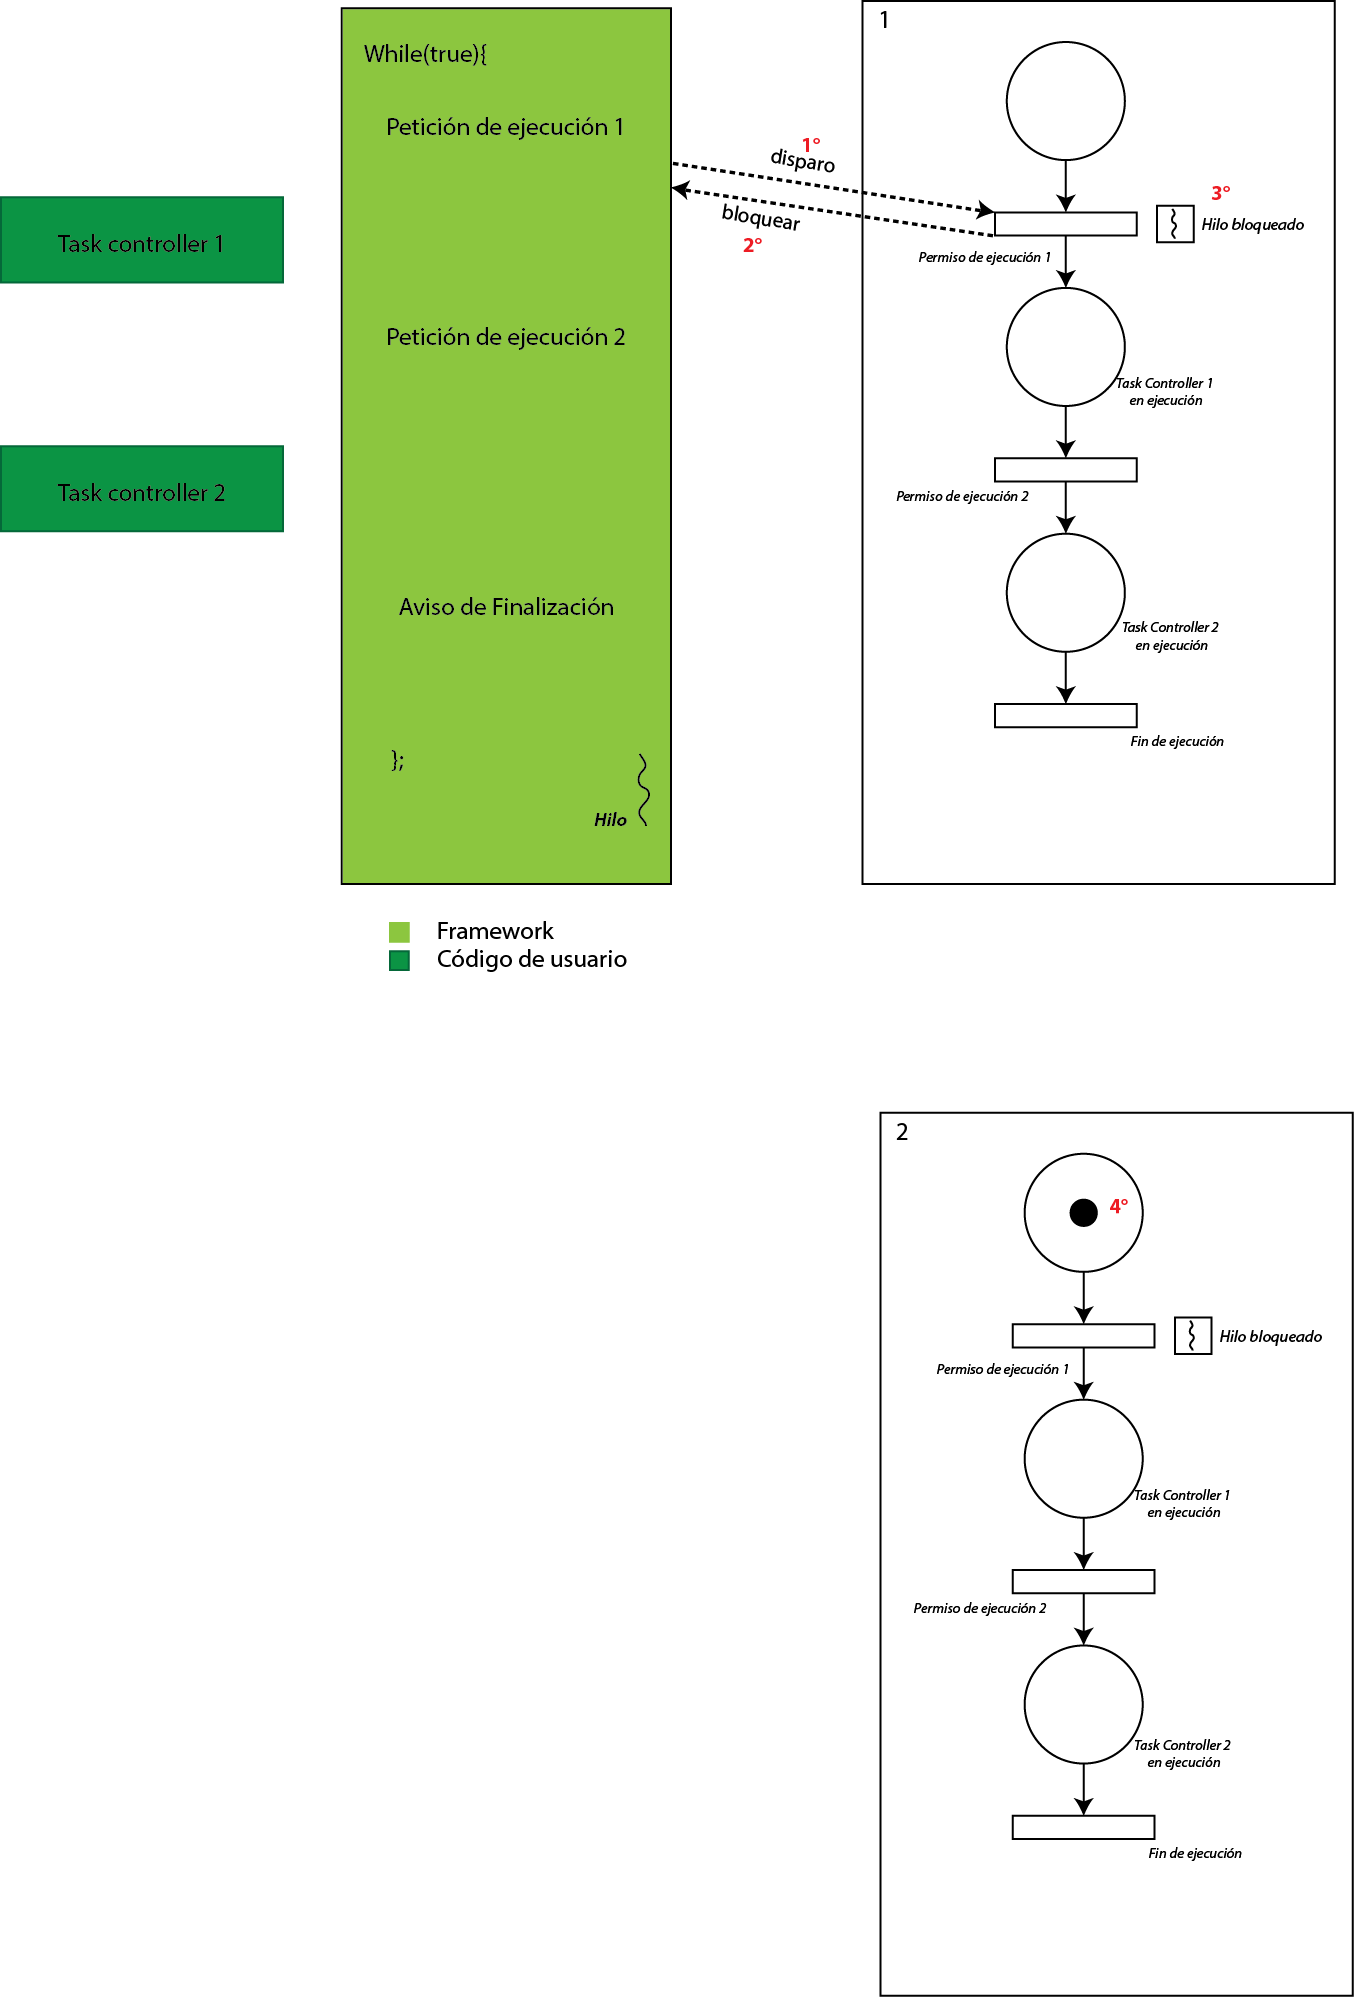
\includegraphics[width=120mm]{ejecucion_complextask_controller_pt1}
\end{figure}

\begin{figure}[H]
	\centering
	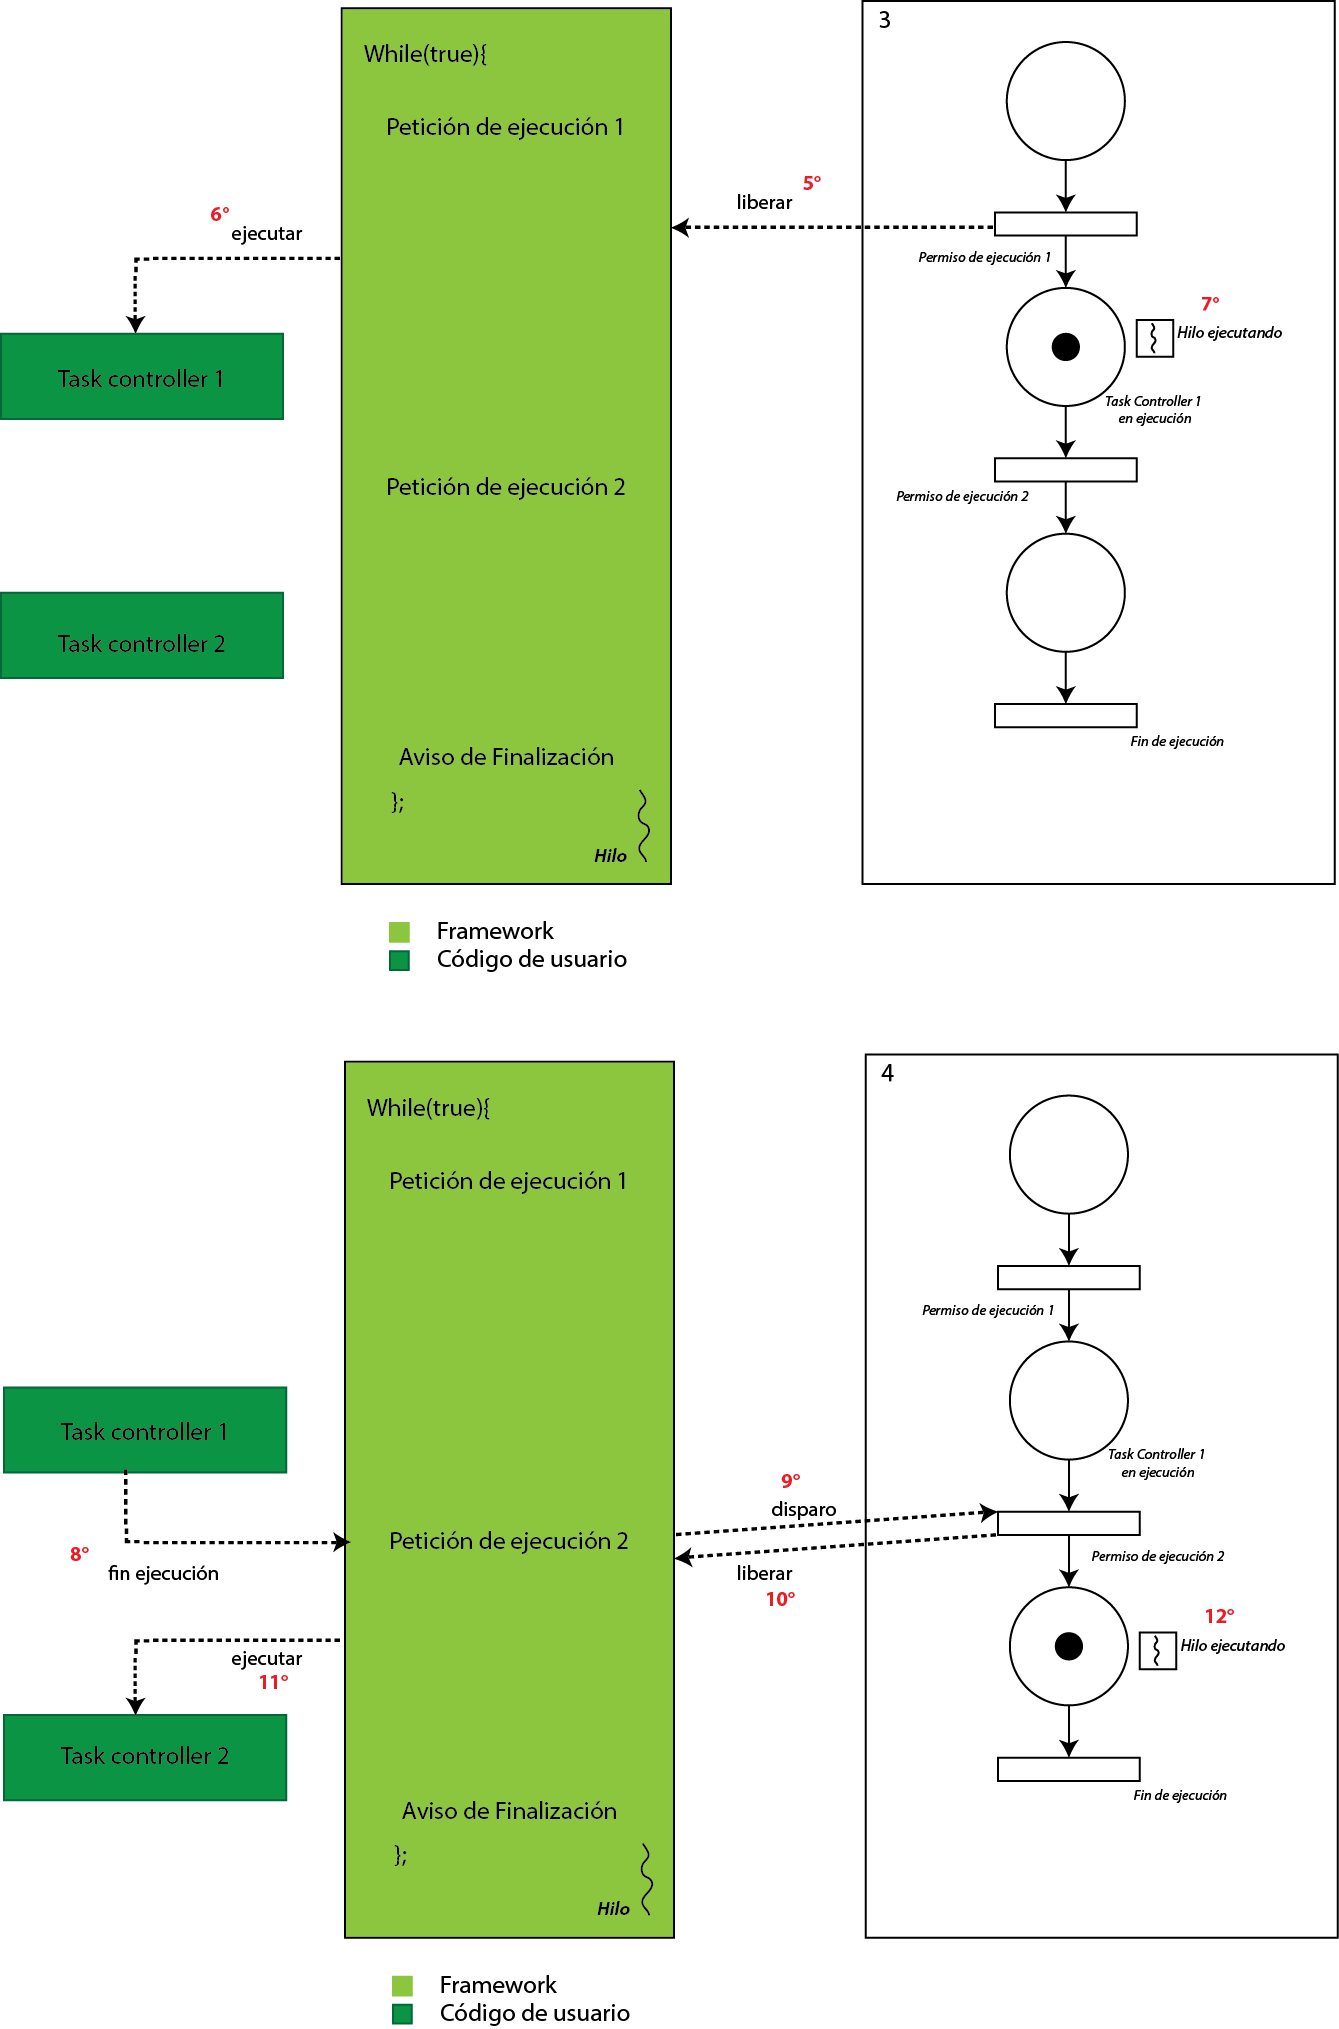
\includegraphics[width=120mm]{ejecucion_complextask_controller_pt2}
\end{figure}

\begin{figure}[H]
	\centering
	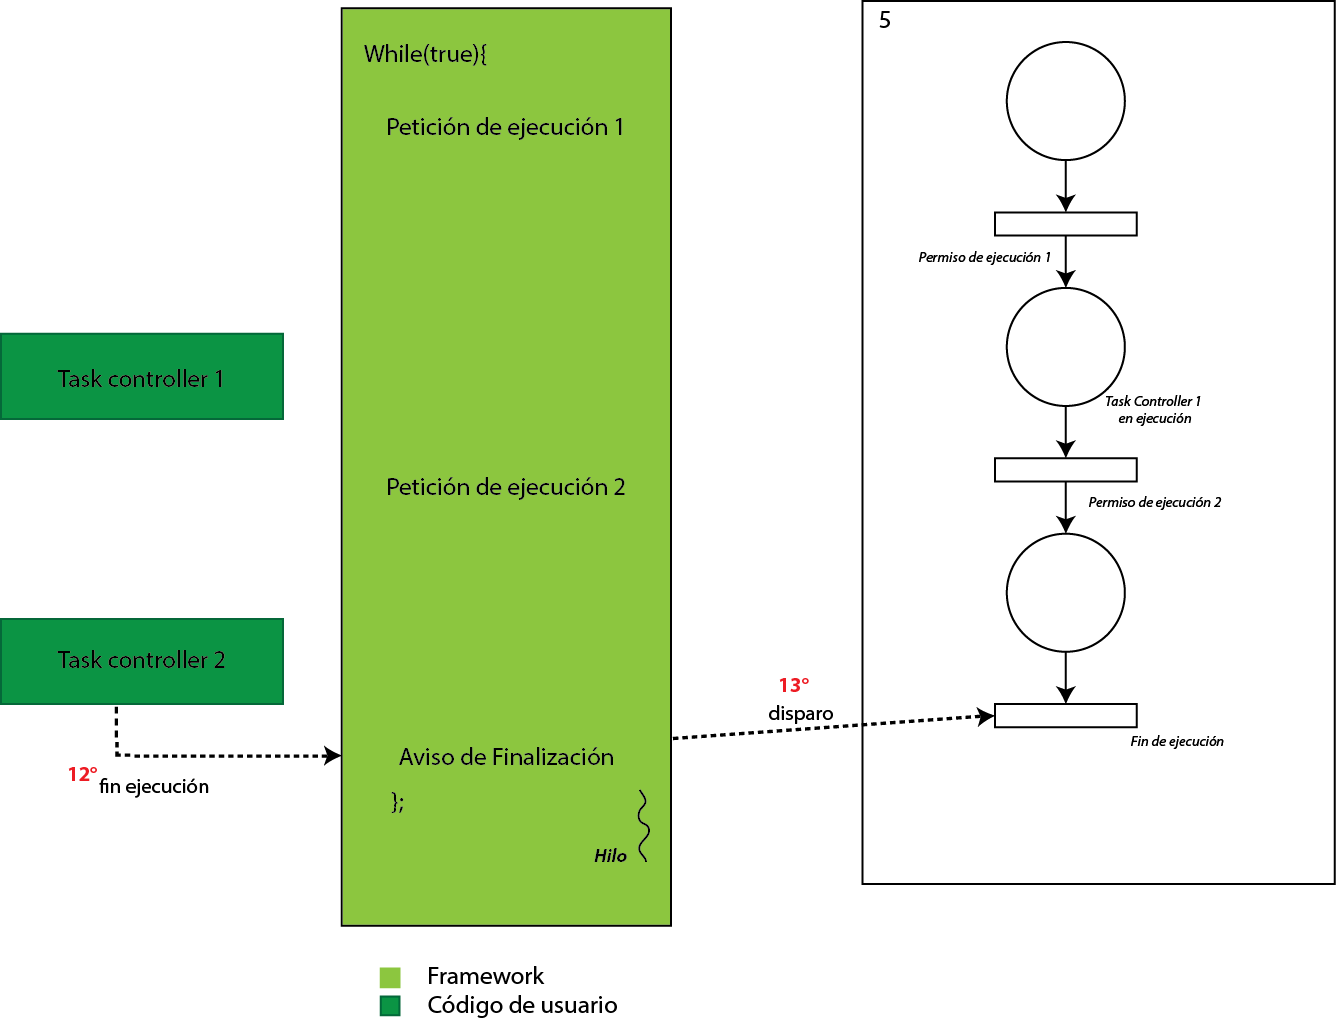
\includegraphics[width=120mm]{ejecucion_complextask_controller_pt3}
	\caption{Pasos de la Ejecución de un Complex Secuential Task Controller con
	Dos Acciones Task}
	\label{fig:ejecucion_complextask_controller}
\end{figure}